% ****** Start of file apssamp.tex ******
%
%   This file is part of the APS files in the REVTeX 4.1 distribution.
%   Version 4.1r of REVTeX, August 2010
%
%   Copyright (c) 2009, 2010 The American Physical Society.
%
%   See the REVTeX 4 README file for restrictions and more information.
%
% TeX'ing this file requires that you have AMS-LaTeX 2.0 installed
% as well as the rest of the prerequisites for REVTeX 4.1
%
% See the REVTeX 4 README file
% It also requires running BibTeX. The commands are as follows:
%
%  1)  latex aps25samp.tex
%  2)  bibtex apssamp
%  3)  latex apssamp.tex
%  4)  latex apssamp.tex
%
\documentclass[%
 reprint,
nofootinbib,
%superscriptaddress,
%groupedaddress,
%unsortedaddress,
%runinaddress,
%frontmatterverbose,
%preprint,
%showpacs,preprintnumbers,
%nofootinbib,
%nobibnotes,
%bibnotes,
aps,
%pra,
%prb,
%rmp,
%prstab,
%prstper,
%floatfix,
]{revtex4-1}

\usepackage[utf8]{inputenc}
\usepackage[english]{babel}
\usepackage{dsfont}
\usepackage{amsmath}
\usepackage{ mathrsfs }
\usepackage{amssymb}
\usepackage{graphicx}% Include figure files
\usepackage{dcolumn}% Align table columns on decimal point
\usepackage{bm}% bold math
\usepackage{amsmath}
\usepackage{varioref}
\usepackage{booktabs}
\usepackage[bottom]{footmisc}

\usepackage{physics}
\usepackage[ruled,vlined]{algorithm2e}
\usepackage{algpseudocode}
\usepackage{listings}

\usepackage{booktabs}

\usepackage{tikz}
\usepackage{float}
\usepackage{siunitx}



\newcolumntype{C}{>{$}c<{$}}
\AtBeginDocument{
\heavyrulewidth=.08em
\lightrulewidth=.05em
\cmidrulewidth=.03em
\belowrulesep=.65ex
\belowbottomsep=0pt
\aboverulesep=.4ex
\abovetopsep=0pt
\cmidrulesep=\doublerulesep
\cmidrulekern=.5em
\defaultaddspace=.5em
}



\usepackage{hyperref}% add hypertext capabilities
%\usepackage[mathlines]{lineno}% Enable numbering of text and display math
%\linenumbers\relax % Commence numbering lines

%\usepackage[showframe,%Uncomment any one of the following lines to test
%%scale=0.7, marginratio={1:1, 2:3}, ignoreall,% default settings
%%text={7in,10in},centering,
%%margin=1.5in,
%%total={6.5in,8.75in}, top=1.2in, left=0.9in, includefoot,
%%height=10in,a5paper,hmargin={3cm,0.8in},
%]{geometry}

\begin{document}


\title{Simulating phase transitions in magnetic systems using the 2D Ising model with the Metropolis algorithm}
\author{Fredrik Hoftun \& Mikkel Metzsch Jensen}

\affiliation{Department of Physics, University of Oslo\\}
\date{\today}



\begin{abstract}
   The aim of the project is to simulate a magnetic phase transition using the widely popular Ising model in two dimensions with the Metropolis algorithm. We started by successfully verifying that our implementation of the model for a $2 \times 2$ lattice were in agreement with the analytical expressions. We then expanded the lattice to a $20\times20$ system and ran calculations of the stabilization time, accepted spin in the Metropolis algorithm as a function of temperature and the energy probability distribution for two different temperatures. We found the general stabilization time to be roughly $10^5$ Monte Carlo cycles depending on the temperature and initial configuration. We saw that the ratio of accepted spins and width of the energy probability distribution increased with temperature. In order to improve the simulation speed we used MPI to parallelize the program yielding a speed-up of approximately $3.6$. We then simulated the phase transition for lattice sizes $L = 40, 60, 80, 100$. As we increased the lattice size we found the result to change towards the analytical expressions at the thermodynamic limit. By scaling our result we found a mean value for the estimated critical temperature for an infinite 2D lattice to be $T_C = 2.269 \pm 0.008 \ k_B/J$. This is consistent with the analytical value by Onsager ($T_C = 2.2692$) within the uncertainties. With this study we have supported the idea that the numerical values are true in the thermodynamic limit.

\end{abstract}

\vfill
\footnotesize{{Link to our GitHub repository: \url{https://github.com/mikkelme/project4_FYS3150}}}
\maketitle
\newpage


\section{Introduction}
The Ising model is a mathematical model that describes ferromagnetism in statistical mechanics. Ferromagnetism is the basic mechanism that makes certain materials (such as iron) magnetizable. The model consist of discretized variables representing the magnetic moment of atomic spins \cite{wiki:Ising}. This is a binary system where each \textit{atom} can have either spin up (+1) or spin down (-1). We put \textit{atom} in italics because we can't possible reach a number of spins in our numerical model that matches the number of atoms in real materials, on the scale of Avogadro's number ($\num{6.022e23}$).\\
In addition to the limitation of only using two dimensions we will also limit our model to a maximum lattice size of $100\times100$ ($10^4$ spins) to limit the simulation time. But as we shall see this might be sufficient to give a comprehensive description of the phase transition which occurs at the critical temperature $T_C$. Such a phase transition describes the change from a state with finite magnetic moment to a state with zero magnetic moment. In other words, the material loses its magnetic properties when heated to the critical temperature. Lars Onsager solved the Ising model in two dimensions analytically in 1944\cite{Onsager} and derived a value for the critical temperature for the infinite 2D lattice. By scaling our result relative to the lattice size we should be able to get a result that is in agreement with the analytic value by Onsager. \\
In this project we are going to implement the Ising model numerically using $\verb!C++!$. We do this by using the Metropolis algorithm with periodic boundary conditions. In order to verify that our implementation is working correctly we will compare our numerical and analytical results for a $2\times 2$ lattice. We will then increase the lattice size to $20\times20$ and make some investigations on the conditions needed for the system to reach equilibrium, the most likely state. In addition we will look at the energy distribution for different temperatures and how this is connected to the acceptance of new energy states in the model. For the final part we will parallelize the code in order to speed-up the simulations so we can handle the more demanding computations. Finally, we will simulate the phase transition for different lattice sizes and compare them to the analytical values of Onsager. We will use the values for heat capacity and magnetic susceptibility to calculate the critical temperature.


\section{Method}
\subsection{Statistical mechanics}
When working with many-particle systems it is unreasonable to study the particles in a microscopical way because of the sheer number of particles. However, it is possible to study such models macroscopically using statistical mechanics. We introduce the canonical ensemble that represent the possible states of a mechanical isolated system in thermal equilibrium with a heat bath at a fixed temperature. \cite{wiki:Canonical_ensemble}. The system can exchange energy with the heat bath but the particle number and volume remain constant. 
 \\
The probability of a state is given by the Boltzmann distribution:
\begin{align*}
    P_i(\beta) = \frac{e^{-\beta E_i}}{Z}, \qquad \beta = 1/k_BT
\end{align*}
where $k_B$ is the Boltzmann constant, $T$ is the temperature, $E_i$ is the energy of microstate $i$ and $Z$ is the partition function which serves as a normalization factor. Since the sum of all probabilities must equal 1 we can easily see that the partition function can be expressed as
\begin{equation}
    Z = \sum_{i = 1}^m e^{-\beta E_i}
    \label{eq:partition}
\end{equation}
where $m$ is the total number of microstates. Note that some energy levels might be degenerate which means that we have to count them multiple times accordingly. \\
We can calculate the expectation value (mean) of a physical value of a discrete distribution as
\begin{align*}
    \langle X \rangle = \sum_{i = 1}^{m} x_i P_i
\end{align*}
Where $\langle X \rangle$ is the expectation value of a variable $X$, $x_i$ is the set of $X$ values and $P_i$ are their probabilities.\newpage This lets us calculate the expectation value of energy $E$ and absolute value of the magnetization $|M|$ as
\begin{align}
    \langle E \rangle &= \frac{1}{Z} \sum_{i = 1}^{m} E_i e^{-\beta E_i} \label{eq:E_num}\\
    \langle |M| \rangle &= \frac{1}{Z} \sum_{i = 1}^{m} |M_i| e^{-\beta E_i} \label{eq:|M|_num}
\end{align}
Note that the $\langle M\rangle$ (without the absolute signs) will equal 0 due to symmetry of microstates with spins pointing up or down.\\ 
The heat capacity at constant volume is given by
\begin{equation}
    C_V = \frac{\sigma_E^2}{k T^2} = \frac{1}{k T^2} (\langle E^2 \rangle - \langle E \rangle^2)
    \label{eq:C_V_num}
\end{equation}
where $\sigma_E$ is the standard deviation of the set of energy values. Similarly, we have the magnetic susceptibility:
\begin{equation}
    \chi = \frac{\sigma_M^2}{k T} = \frac{1}{k T} (\langle M^2 \rangle - \langle |M| \rangle^2)
    \label{eq:chi_num}
\end{equation}
where $\sigma_M$ is the standard deviation of the set of magnetization values.

\subsection{The Ising model}
The energy of the two dimensional Ising model, without an external magnetic field, is given as:
\begin{equation}
    E = -J \sum_{<kl>}^N s_ks_l
    \label{eq:Ising_energy}
\end{equation}
where the spins $s_k$ and $s_l$ can take values $\pm1$ for up and down spins. N is the total number of spins and $J$ is a coupling constant expressing the strength of the interaction between neighbouring spins. The $<kl>$ notation means that we only sum over nearest neighbours to index l. For a two dimensional lattice this would mean that we consider the neighbour spins at the left, right, bottom and top. Another property is the total magnetization $M$ which can be found by summing over individual spins as 
\begin{equation}
    M = \sum_{j=1}^N s_j
    \label{eq:Ising_magnetization}
\end{equation}
In general we see that aligned spin gives raise to a magnetization while disaligned does not. 

\subsection{Phase transitions and the Onsager limit}
Phase transitions make materials undergo fundamental changes. During a phase transition (for temperatures near $T_C$), the expectation value of the magnetization is given by:
\begin{align*}
    \langle M \rangle \sim (T- T_C)^{\beta}, \quad \beta = 1/8
\end{align*}
where $T_C$ is the critical temperature, the temperature where a phase transition occurs and $\beta$ is the critical exponent. The heat capacity and magnetic susceptibility is given by:
\begin{align*}
    C_V &\sim |T_C - T|^{\alpha}, \quad \alpha = 0\\
    \chi &\sim |T_C - T|^{\gamma}, \quad \gamma = 7/4
\end{align*}
\newpage As the temperature rises and approaches the critical temperature $T_C$, the individual spins become more and more correlated. This gives rise to a new quantity called the correlation length, $\xi$. Close to the critical temperature the correlation length is:
\begin{align*}
    \xi &= |T_C - T|^{-\nu} \propto L
\end{align*}
Since the correlation length is proportional to the lattice size we can rewrite our equations above:
\begin{align*}
    \langle M \rangle &\propto L^{-\beta /\nu}\\
    C_V &\propto L^{\alpha /\nu}\\
    \chi &\propto L^{\gamma /\nu}
\end{align*}
By using so-called finite size scaling relations it is possible to relate the behaviour of the finite lattice with the behaviour of an infinte lattice as:
\begin{equation}
    T_C(L) - T_C(L=\infty) = aL^{1/\nu}
    \label{eq:lattice scaling}
\end{equation}
 In Onsager's two dimensional Ising model solution, he used the fact that the correlation length is proportional to the lattice size, with $\nu = 1$, to calculate the critical temperature
\begin{align*}
    \frac{k T_C}{J} &= \frac{2}{\ln{(1+\sqrt{2})}} \approx 2.2692
\end{align*}
If we use $\nu = 1$ in equation \ref{eq:lattice scaling} we can describe it as a linear relationship
\begin{equation}
    T_C(L) = a\frac{1}{L} + T_C(L=\infty)
    \label{eq:findTc}
\end{equation}

\subsection{Algorithm}
In order to simulate the Ising model we will use the Monte Carlo (MC) sampling based Metropolis algorithm. The Metropolis algorithm considers only ratios between probabilities and we do not need to compute the partition function which require us to know all states. For a $L\times L$ lattice with a total of $N=L^2$ spins we have a total of $m=2^N$ microstates. For a lattice of size $L = 100$ this would result in $10^{3010}$ microstates which is clearly out of the range for computational practice. The relative probability of two states 1 and 2 are given as:
\begin{align*}
    \frac{P_1}{P_2} = \frac{Z}{Z} \frac{e^{-\beta E_1}}{e^{-\beta E_2}} = e^{\beta (E_2 - E_1)}
\end{align*}
The metropolis algorithm uses the following procedure for a $L\times L$ lattice.
\begin{itemize}
    \item Choose a random spin among the N spins in the $L\times L$ lattice
    \item Calculate the energy difference $\Delta E = E_{new} - E_{old}$ if the spin were to be flipped.
    \item We accept the new configuration if $\Delta E \leq 0$ or if the relative probability $P_{old}/P_{new}$ is less or equal to a random value $r$ between 0 and 1. The acceptance condition can be written as
    \begin{align*}
        e^{\beta \Delta E} \leq r
    \end{align*}
    This accounts for random flips in the lattice.
    \item If the new configuration is accepted, update the total energy and magnetization.
\end{itemize}
This is repeated $N=L^2$ times to constitute one sweep over the lattice, which is then repeated for as many Monte Carlo cycles (MC cycles) as possible.
\newpage
\subsubsection{Determining the energy differences for the Metropolis algorithm}\label{sec:energy_change}
In order to implement this effectively we can use that the change in energy when performing a flip $\Delta E$ only have a limited set of possible values. We look at the case of flipping only one spin, from spin state 1 to 2, while the neighbours remain constant. By the use of equation \ref{eq:Ising_energy} we can calculate the energy difference as
\begin{align*}
    \Delta  = E_2 - E_1 =& -J \sum_{<kl>}^N s_k^2s_l^2 + J \sum_{<kl>}^N s_k^1s_l^1
\end{align*}
where $s_l^i$ is the middle spin (the one we flip) in state $i$ and $s_k^i$ is the neighbour spin in state $i$. Since we only change $s_l$ we can use $s_k^1 = s_k^2$ and rewrite as
\begin{align*}
    \Delta E = -J \sum_{<kl>}^N s_k^2s_l^2 + J \sum_{<kl>}^N s_k^2s_l^1 = -J\sum_{<kl>}^N s_k^2(s_l^2 - s_l^1)
\end{align*}
The spin to be flipped only take values $s_l^1 \pm 1$ and we have $s_l^2 = - s_l^1$ which gives
\begin{align*}
    (s_l^2 - s_l^1) = - s_l^1 - s_l^1 = -2s_l^1
\end{align*}
This lead to the final expression:
\begin{equation}
     \Delta E  = -J\sum_{<kl>}^N -s_k^2 2s_l^1 = 2Js_l^1\sum_{<k>}^N s_k
     \label{eq:Delta_E}
\end{equation}
where we dropped the state indicator on $s_k$ since the neighbour spins are unchanged. \\
The change in magnetisation when flipping one spin is simply given as:
\begin{align*}
    \Delta M = M_2 - M_1 = s_l^2 - s_l^1 = -2s_l^1 = 2s_l^2
\end{align*}
This can also be expressed as:
\begin{align*}
    M_2 = M_1 + 2s_l^2
\end{align*}
With the use of equation \ref{eq:Delta_E} we can calculate the five possible values for the energy change. When flipping the middle spin from up to down (1 to -1) in the following configurations we get the energy differences as shown here:
\begin{align*}
    &\begin{pmatrix} &\uparrow&\\ \uparrow&\uparrow&\uparrow\\ &\uparrow&\\\end{pmatrix}_1 \ \Longrightarrow
    \begin{pmatrix} &\uparrow&\\ \uparrow&\downarrow&\uparrow\\ &\uparrow&\\\end{pmatrix}_2 \qquad
    \Delta E = 2J\cdot4 = 8J& \\
    &\begin{pmatrix} &\uparrow&\\ \downarrow&\uparrow&\uparrow\\ &\uparrow&\\\end{pmatrix}_1 \ \Longrightarrow
    \begin{pmatrix} &\uparrow&\\ \downarrow&\downarrow&\uparrow\\ &\uparrow&\\\end{pmatrix}_2 \qquad
    \Delta E = 2J\cdot2 = 4J& \\
    &\begin{pmatrix} &\downarrow&\\ \downarrow&\uparrow&\uparrow\\ &\uparrow&\\\end{pmatrix}_1 \ \Longrightarrow
    \begin{pmatrix} &\downarrow&\\ \downarrow&\downarrow&\uparrow\\ &\uparrow&\\\end{pmatrix}_2 \qquad
    \Delta E = 2J\cdot0 = 0& \\
    &\begin{pmatrix} &\downarrow&\\ \downarrow&\uparrow&\uparrow\\ &\downarrow&\\\end{pmatrix}_1 \ \Longrightarrow
    \begin{pmatrix} &\downarrow&\\ \downarrow&\downarrow&\uparrow\\ &\downarrow&\\\end{pmatrix}_2 \qquad
    \Delta E = 2J\cdot(-2) = -4J& \\
    &\begin{pmatrix} &\downarrow&\\ \downarrow&\uparrow&\downarrow\\ &\downarrow&\\\end{pmatrix}_1 \ \Longrightarrow
    \begin{pmatrix} &\downarrow&\\ \downarrow&\downarrow&\downarrow\\ &\downarrow&\\\end{pmatrix}_2 \qquad
    \Delta E = 2J\cdot(-4) = -8J& \\
\end{align*}
We see that it is symmetrical such that a change in spin from down to up will grant the same values but in reversed order. Since the energy difference only depends on the sum of the neighbouring spins, we do not have to worry about multiplicity. The five possible values for the energy change is thereby given as
\begin{equation}
    \Delta E = \{8J, 4J, 0, -4J, -8J\}
    \label{eq:Delta_E_list}
\end{equation}
\newpage
\subsubsection{Implementation of random values}
Since a computer is deterministic it cannot generate true random numbers, only pseudo random numbers. Our algorithm will at most do $10^6$ MC cycles on a maximum lattice of $100 \times 100$ spins, resulting in $10^{10}$ loops. This means that our random number generator (RNG) must have a period $P$ larger than the total number of loops $P > 10^{10}$. We will use the Mersenne Twister, a fast RNG which has a period of $P = 2^{19937}-1 \approx 10^{6001} >> 10^{10}$. The Mersenne Twister is implemented in $\verb!C++!$ in the $<random>$ library.

\subsubsection{Initial state and equilibration time}
In order to use the Metropolis algorithm we must decide on a starting configuration for the system. Here the natural choices are either to put all spins up or down (same direction) or to put them up and down randomly. The idea is that we should choose the starting point closest to the most likely state. This will in theory reduce the time (number of MC cycles) needed for the system to stabilize. For low temperatures the most likely state will have spins aligned while the spins will be disaligned for higher temperatures. Therefore a default choice could be all spins up for $T < 1.5 \ k_B/J$ and a random configuration when $T > 1.5 \ k_B/J$.\\
Even though we implement a dynamic starting configuration depending on temperature the system will still use a lot of cycles to reach the most likely state. When calculating the expectation values for the phase transition we do not want to include data from the stabilization period. One way to solve this problem is to simply exclude this part of the data in the calculations. In order to know where to make the cut we would then have to study the model in action and make a rough estimate of the stabilization time. Another more advanced solution would be to implement an algorithm that recognizes when the system have reached the most likely state. By analyzing the change in the expectation values for energy and magnetization one could make a threshold for marking the most likely state. When this is reached we can start the gathering of data. Such an algorithm might be to complicated when considering the large fluctuations that happens during the MC cycles. In addition such an algorithm might take up a lot of CPU time. For this project we choose the first and simpler strategy. 

\subsubsection{Boundary conditions}
While real-life systems have numbers of particles in the order of Avogadro's number, $N_A \propto 10^{23}$, we can't reach such numbers using numerical models. Our numerical solution is capped at a lattice size of $100 \times 100 = 10^4$ particles. We can mitigate this problem by implementing periodic boundary conditions where we latch the outer rows to each-other. For a one dimensional system, a line of spins, we can think of this as gluing the endpoints together such that every spin has two neighbours. In order to implement the periodic boundary conditions effectively for the 2D system in the model, we expand the matrix that holds the lattice from a $L\times L$ to a $(L+1) \times (L+1)$ matrix. By adding this rim around the lattice we can then copy the values on the edge of the lattice to the opposite free space. By doing that we ensure that the edge of the lattice sees the correct neighbour as illustrated in figure \ref{fig:periodic_boundary}. Note that the outer rim should not be seen as a part of the system but purely as a practical implementation of the periodic boundary conditions. Alternatively one could use free ends where we simply ignore contributions from outside the endpoints, this however is more prone to uncertainty. 
 \begin{figure}  
    \centering
    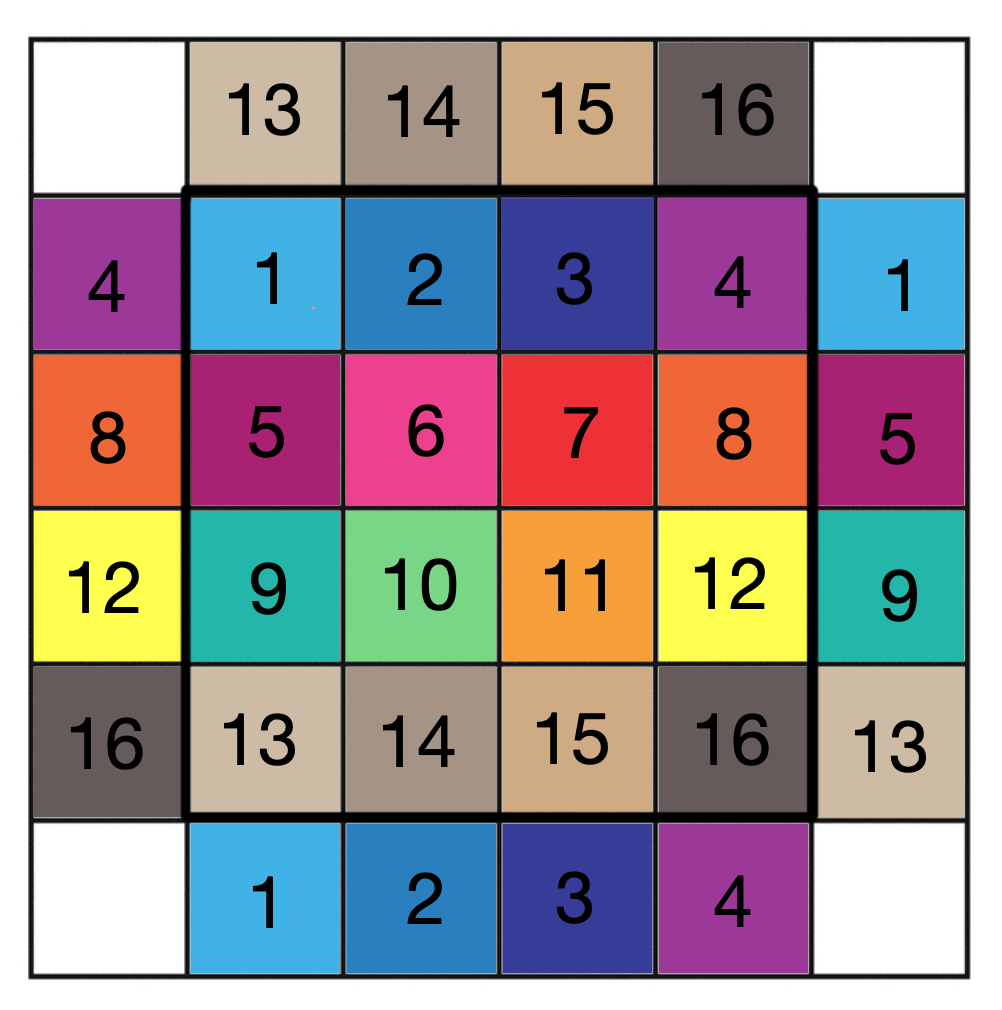
\includegraphics[width=0.45\textwidth]{figures/periodic_boundary.png}
    \caption{Visualization of how the periodic boundary conditions are implemented. It shows the matrix for a $4\times4$ lattice with 16 spins. The inner square (the actual lattice) is extended such that the outer layer contains the effective neighbours according to the periodic boundary conditions. For instance, we see that the right side of the matrix (4, 8, 12, 16) now sees the left side (1, 5, 9, 13) as neighbours and vice versa.}
    \label{fig:periodic_boundary}
\end{figure}

\subsubsection{Optimization}
One of the crucial parts for the effectiveness of the Metropolis algorithm is the calculation of ratios of probability expressed in the passing criteria:
\begin{align*}
    e^{\beta \Delta E} \leq r
\end{align*}
As we have seen in section \ref{sec:energy_change}, $\Delta E$ can take only five values (see equation \ref{eq:Delta_E_list}) which means that we can pre-calculate the above expression for each temperature and store it as an array. This saves 3 FLOPs for each round of the Metropolis algorithm. Since this is called $N$ times for each MC cycle this makes a big difference in computation time.\\
Another issue is that as the lattice size $L$ is increased, the time it takes to compute the algorithm is increased by a factor $L^2$. Since we generally use $10^6$ MC cycles this will make the simulations on big systems very time-consuming. This can be partially mitigated by numerical parallelization, meaning that we can split the work onto different processing units (cores). Our best resource for the simulations was a MacBook Pro 2020, 2.3 GHz Quad-core Intel Core i7. This has the potential to grant a speed-up of a factor four when parallelized properly. 


\subsection{Units}
We will be using natural units of $k_B$ and $J$. This makes the results easier to visualize and also mitigates eventual issues with numerical precision. In our system of units, energy has unit $J$ (order of coupling constant, not joules), temperature has $k_B/J$, heat capacity has $k_B$, magnetic susceptibility has $1/J$ and the magnetization is unit-less. 
\newpage
\section{Results}
The styling on our figures is inspired from another GitHub repository\cite{fig:style}.
\subsection{2 x 2 lattice - analytical results.}\label{sec:analytical}
First we took a look at the simple case of the 2 x 2 lattice. This means that we have four spins which is either spin up (+1) or spin down (-1). In total this gives $m = 4^2= 16$ possible microstates, which can be written out as follows.
\begin{align*}
1=\ &\begin{matrix}\uparrow&\uparrow\\\uparrow&\uparrow \end{matrix}& \\
2=\ &\begin{matrix}\downarrow&\uparrow\\\uparrow&\uparrow \end{matrix}&
3=\ &\begin{matrix}\uparrow&\downarrow\\\uparrow&\uparrow \end{matrix}&
4=\ &\begin{matrix}\uparrow&\uparrow\\\downarrow&\uparrow \end{matrix}&
5=\ &\begin{matrix}\uparrow&\uparrow\\\uparrow&\downarrow \end{matrix}&\\
6=\ &\begin{matrix}\uparrow&\uparrow\\\downarrow&\downarrow \end{matrix}&
7=\ &\begin{matrix}\downarrow&\downarrow\\\uparrow&\uparrow \end{matrix}&
8=\ &\begin{matrix}\downarrow&\uparrow\\\uparrow&\downarrow \end{matrix}&
9=\ &\begin{matrix}\uparrow&\downarrow\\\downarrow&\uparrow \end{matrix}&
10=\ &\begin{matrix}\uparrow&\downarrow\\\uparrow&\downarrow \end{matrix}&
11=\ &\begin{matrix}\downarrow&\uparrow\\\downarrow&\uparrow \end{matrix}&\\
12=\ &\begin{matrix}\uparrow&\downarrow\\\downarrow&\downarrow \end{matrix}&
13=\ &\begin{matrix}\downarrow&\uparrow\\\downarrow&\downarrow \end{matrix}&
14=\ &\begin{matrix}\downarrow&\downarrow\\\uparrow&\downarrow \end{matrix}&
15=\ &\begin{matrix}\downarrow&\downarrow\\\downarrow&\uparrow \end{matrix}&\\
16=\ &\begin{matrix}\downarrow&\downarrow\\\downarrow&\downarrow \end{matrix}&
\end{align*}
By using equation \ref{eq:Ising_energy} we calculated the energies for all these microstates separately. For this we used periodic boundary conditions and were careful not to count the connections between spin twice. Below are some of the calculation showcased:
\begin{align*}
    &E_1 = E_{16} = 2 \cdot (-4J) = -8J& &E_2 = 4J - 4J = 0& &E_8 = E_9 = 2 \cdot 4J&
\end{align*}
In addition we calculated the magnetization $M_i$ for a given configuration using equation \ref{eq:Ising_magnetization}. The resulting energies and magnetizations are ordered and presented in table \ref{tab:2x2_EM}.
\begin{table}[H]
  \begin{center}
  \caption{Energy and Magnetization for all possible configurations of the $4\times 4$ lattice}
  \begin{tabular}{|c|c|c|c|} \hline
  \textbf{No. of spins up} & \textbf{Degeneracy} & \textbf{Energy} & \textbf{Magnetization} \\ \hline
  4 & 1 & -8J & 4 \\ \hline
  3 & 4 & 0 & 2 \\ \hline
  2 & 4 & 0 & 0 \\ \hline
  2 & 2 & 8J & 0 \\ \hline
  1 & 4 & 0 & -2 \\ \hline
  0 & 1 & -8J & -4 \\ \hline
  \end{tabular}
  \label{tab:2x2_EM}
  \end{center}
\end{table}
Then we used equations \ref{eq:partition}, \ref{eq:E_num}, \ref{eq:|M|_num}, \ref{eq:C_V_num} and \ref{eq:chi_num} to calculate the partition function $Z$ and the expectation value for: The energy $E$, energy squared $E^2$, absolute magnetization $|M|$ and magnetization squared $M^2$, along with the heat capacity $C_V$ and magnetic susceptibility $\chi$.
\begin{align*}
    Z &= 4\cosh{8J\beta} + 12 \\
    \langle E \rangle &= \frac{-32J\sinh{8J\beta}}{Z} \\
    \langle E^2 \rangle &= \frac{256J^2 \cosh{8J\beta}}{Z} \\
    \langle|M|\rangle  &= \frac{8e^{8J\beta} + 16}{Z} \\
    \langle M^2 \rangle &= \frac{32e^{8J\beta} + 32}{Z} \\
    C_V &= \frac{32J^2}{kT^2}\frac{8\cosh{(8J\beta)}Z -32\sinh^2{(8J\beta)}}{Z^2} \\
    \chi &= \beta\left(32\frac{e^{8J\beta} + 1}{Z} - (\frac{8e^{8J\beta} + 16}{Z})^2\right) 
\end{align*}

\subsection{2x2 benchmark - Comparing numerical and analytical results}\label{sec:2x2}
We used the analytical results calculated in section \ref{sec:analytical} to test our numerical calculations. In our test-case we initialized the system with a temperature $T = 1.0 \ k_B/J$ and pointed all the spins upwards. We then ran $10^6$ MC cycles while computing the expectation values per spin for the energy, energy squared, absolute magnetization and magnetization squared, as well as computing the heat capacity and magnetic susceptibility of the system. The results are displayed in figure \ref{fig:equilibrium_benchmark}. We observe that the numerical values approach the analytical ones as the number of cycles increases during the simulation.\\
We also plotted the computed values, during $10^6$ MC cycles, as a function of temperature to verify that the they match the analytical functions. This is shown in figure \ref{fig:phase_benchmark}.

\onecolumngrid

\begin{figure}[H]
  \centering
  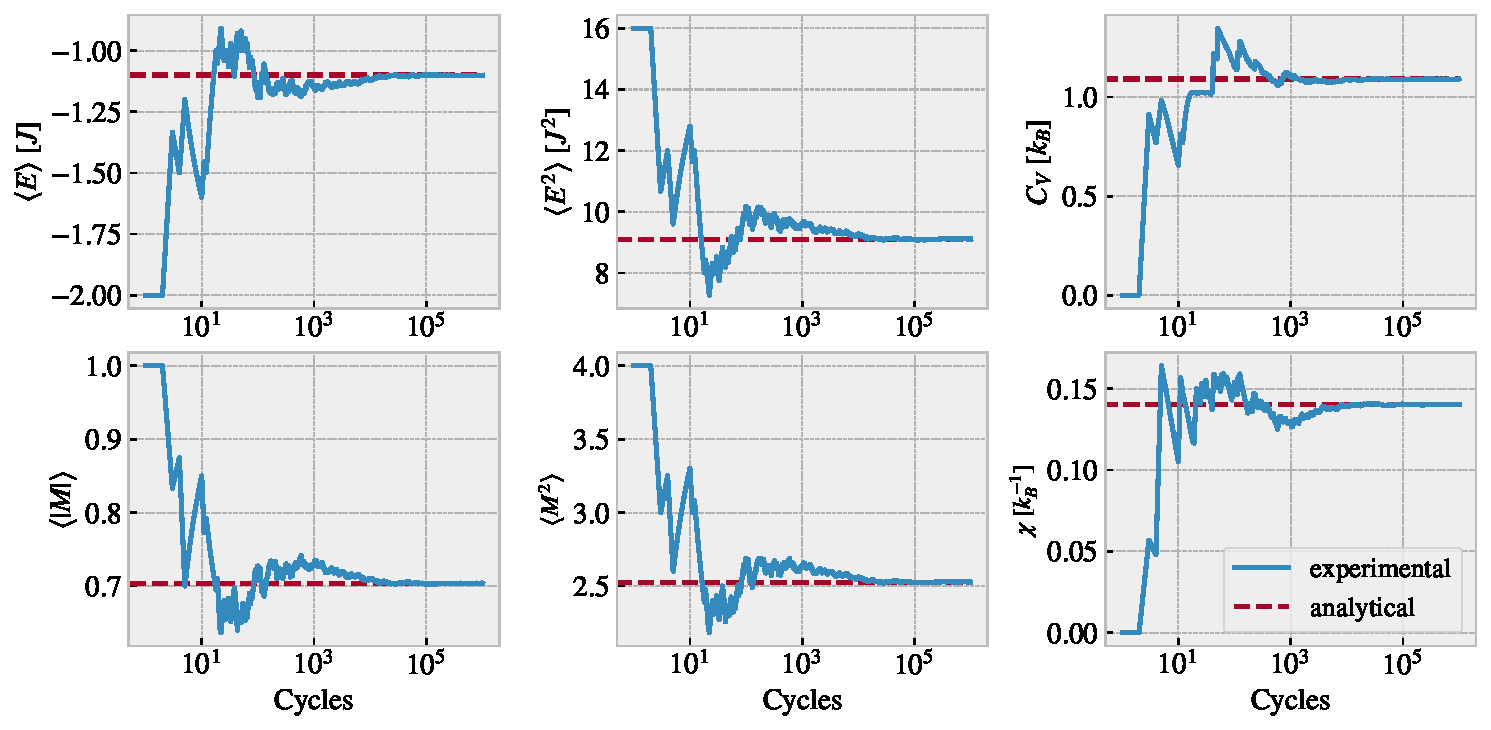
\includegraphics[width=0.8\textwidth]{figures/equilibrium_benchmark.pdf} 
  \caption{The expectation values per spin for: energy $E$, energy squared $E^2$, absolute magnetization $|M|$, magnetization squared $M^2$ and the heat capacity $C_V$ and susceptibility $\chi$ as a function of MC cycles on a $2\times2$ lattice. The blue line shows numerical results while the red dotted line indicates the expected analytical values found in section \ref{sec:analytical}. We initialized the system in a configuration with all spins up and a temperature $T = 1.0$ $[k_B/J]$ and let it run for a total of $10^6$ MC cycles. As the system stabilized we observe that the numerical values approach the analytical values.}
  \label{fig:equilibrium_benchmark}
\end{figure}
\begin{figure}[H]
  \centering
  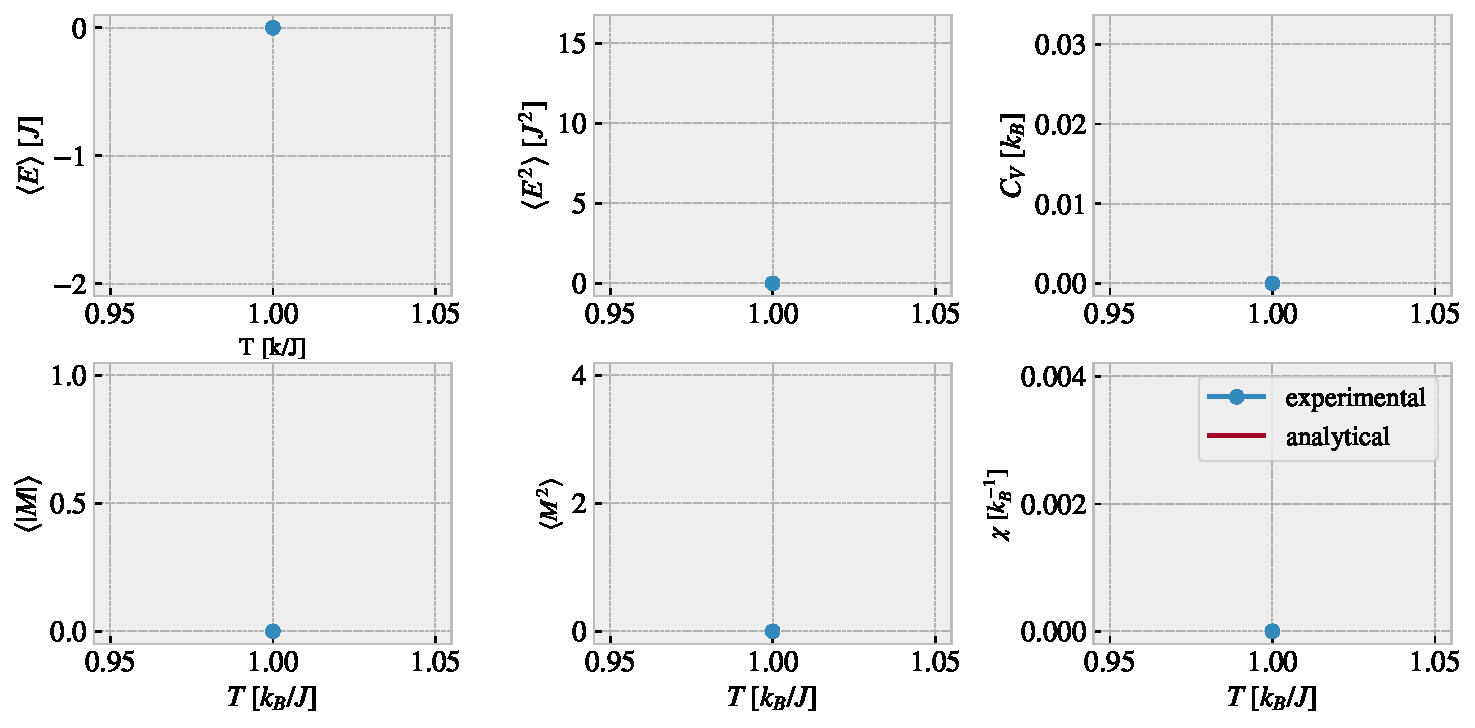
\includegraphics[width=0.8\textwidth]{figures/phase_benchmark.pdf}
  \caption{The expectation values per spin for: energy $E$, energy squared $E^2$, absolute magnetization $|M|$, magnetization squared $M^2$ and the heat capacity $C_V$ and susceptibility $\chi$ as a function of temperature on a $2\times2$ lattice. The values are computed for a \textit{run time} of $10^6$ MC cycles for each temperature step. The blue dots show the numerical data while the red line represents the analytical results. The system was initialized with all spins up for each temperature.}
  \label{fig:phase_benchmark}
\end{figure}

% \clearpage
\newpage
\twocolumngrid



\subsection{Reaching equilibrium}
After having tested our numerical implementation in section \ref{sec:2x2} we expanded the system to a $20 \times 20$ lattice. The intention was to observe how systems with different initial conditions stabilize and approach equilibrium. We ran four different simulations by changing temperature and initial configuration; two simulations for $T = 1.0 \ k_B/J$, one with an initial configuration where all spins pointed up and one with spin direction randomized. We did the same for $T = 2.4 \ k_B/J$. We then calculated the expectation values per spin for the energy and the absolute magnetization, shown in figure \ref{fig:equilibrium_energy} and \ref{fig:equilibrium_magnetization}.\\
We also investigated how the number of accepted flips was affected by the temperature. We used random spin direction for the initial configuration and ran $10^6$ MC cycles for different temperatures. We then calculated the ratio between the number of accepted spins and total spin-flips proposed ($20^2 \times 10^6 = \num{4e8}$) as a function of temperature, shown in figure \ref{fig:accepted_spins}.
\hfill \linebreak
\hfill \linebreak
\hfill \linebreak
\hfill \linebreak
\hfill \linebreak
\hfill \linebreak

 \begin{figure}[H]  
  \centering
  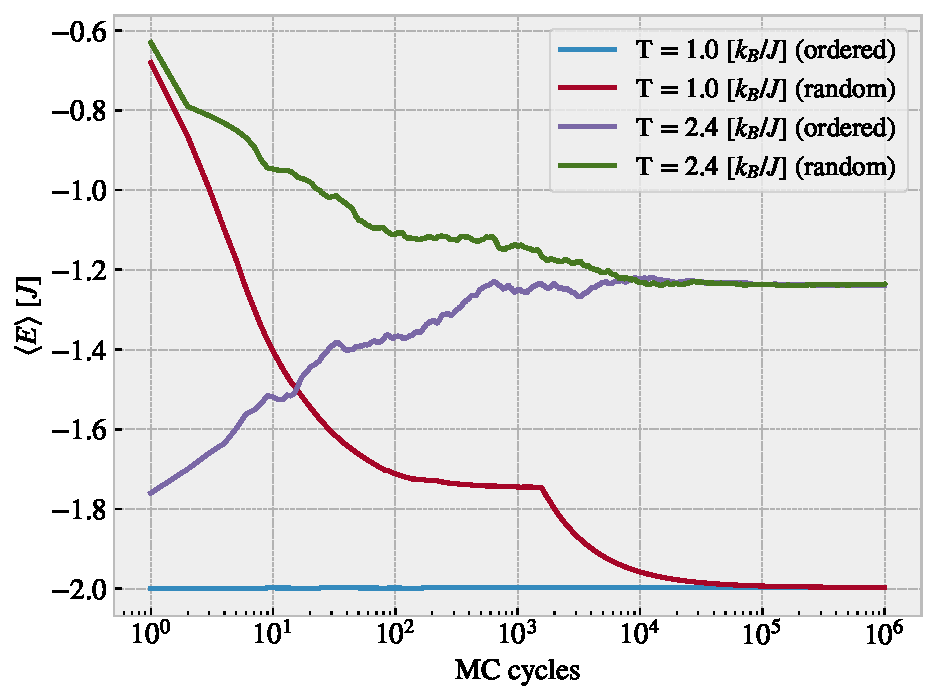
\includegraphics[width=0.45\textwidth]{figures/equilibrium_energy.pdf}
  \caption{The expectation value of the energy $E$ per spin for a $20\times20$ lattice with different initial conditions. We ran four different simulations by changing temperature and initial configuration as showed on the figure. \textit{Ordered} refer to an initial configuration where all spins pointed up and \textit{random} refers to an initial configuration with spin direction randomized. We let the simulation run for $10^6$ MC cycles to study the equilibrium time (given in number of cycles) and the effect of the starting configuration.}
  \label{fig:equilibrium_energy}
\end{figure}

\hfill \linebreak

 \begin{figure}[H]  
  \centering
  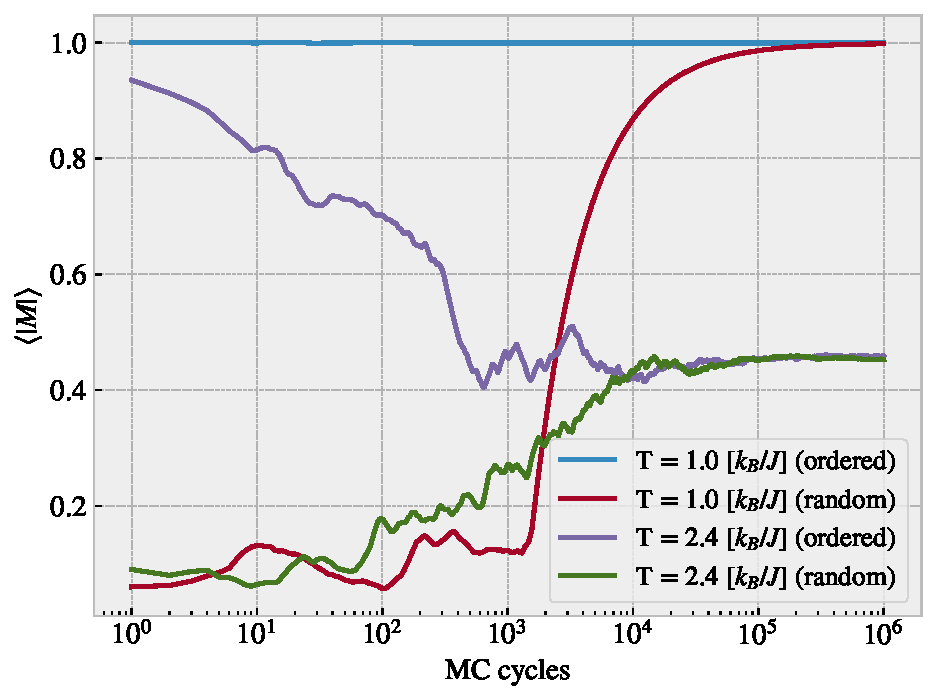
\includegraphics[width=0.45\textwidth]{figures/equilibrium_magnetization.pdf}
  \caption{The expectation value of the absolute magnetization $|M|$ per spin for a $20\times20$ lattice with different initial conditions. We ran four different simulations by changing temperature and initial configuration as showed on the figure. \textit{Ordered} refer to an initial configuration where all spins pointed up and \textit{random} refers to an initial configuration with spin direction randomized. We let the simulation run for $10^6$ MC cycles to study the equilibrium time (given in number of cycles) and the effect of the starting configuration.}
  \label{fig:equilibrium_magnetization}
\end{figure}

 \begin{figure}[H]  
  \centering
  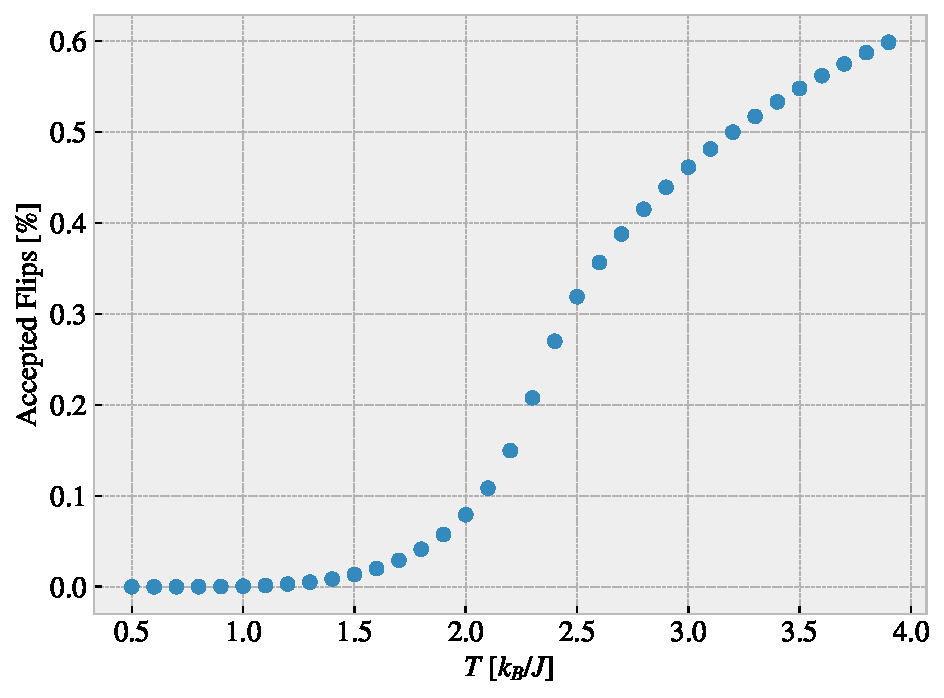
\includegraphics[width=0.45\textwidth]{figures/accepted_flips.pdf}
  \caption{The number of accepted flips (by the Metropolis algorithm) for a series of simulations with different temperatures at $10^6$ MC cycles. We initialized the lattice with random spin direction for each temperature. The number of accepted flips is given as a ratio between the number of flips and the total number of flip proposals ($\num{4e8}$). In this particular case the stabilization period in the beginning is included in the data.}
  \label{fig:accepted_spins}
\end{figure}


\clearpage
\subsection{Probability distribution}
We have computed the energy probability distribution for temperatures 1.0 and 2.4 $k_B/J$ by simply counting the number of times a given energy appears during the simulation. We used $L = 20$ and $10^6$ MC cycles. We did not gather data from the first $10^4$ cycles as we assumed this to be a reasonable estimate for the cycles needed to reach the most likely state. The results are shown as a normalized histogram in figure \ref{fig:energy_distribution}.
 \begin{figure}[H]  
  \centering
  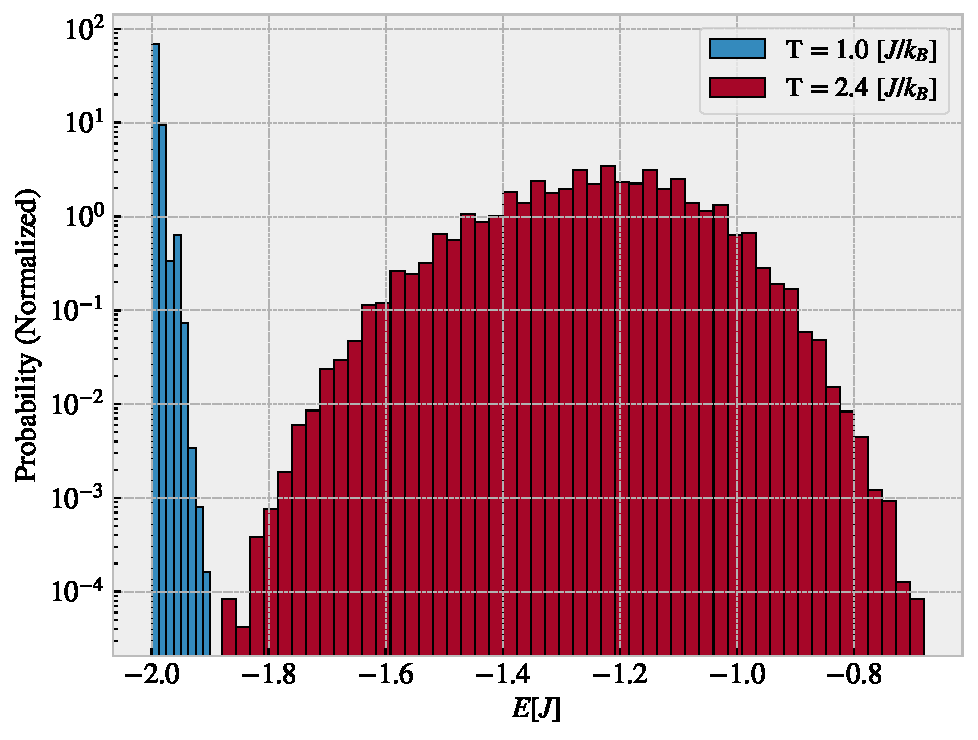
\includegraphics[width=0.45\textwidth]{figures/probability_distribution.pdf}
  \caption{The energy per spin probability distribution for a $20\times20$ lattice simulated at different temperatures. The distribution is found by simply counting the number of times a given energy appears and dividing with the total number of energies to normalize the results. The results are showed as a histogram with a bin width of 8 for $T = 1$ and a bin width of 50 for $T = 2.4$. We initialized the system with all spins up for the low temperature and random spin direction for the highest temperature. The simulation ran for $10^6$ MC cycles. The data from the first $10^4$ cycles were excluded from the calculation due to the stabilization time.} 
  \label{fig:energy_distribution}
\end{figure}


\subsection{Timing of algorithm}
We have performed time measurements of the simulation, with and without parallelization. We did this by varying the number of MC cycles, total number of spins $N$ and temperature individually. The default values when not varied were put to $10^6$ MC cycles, 400 spins ($L = 20$) and $T = 1 \ k_B/J$. We ran the simulation on a Macbook Pro 2020 2.3 GHz Quad-Core Intel core i7 and we wanted to see how much of a  speed-up we achieved when using all four cores (parallelized) instead of just one core (not parallelized). We disabled writing to file and other unnecessary computations during the simulation. We only timed the program during the run through of the main algorithm after the initial stabilization. By varying each of the values individually we produced the results showed in figure \ref{fig:tmMCcycles}, \ref{fig:tmSpins} and \ref{fig:tmTemp}. By performing linear regression on the data as a function of number of MC cycles and number of spins we verified that the time used was linearly dependent on both of these variables. By comparing the slopes we estimated the speed-up by parallelization as showed in table \ref{tab:timing_results}. For the case of the change in temperature we saw a non-linear dependency between the time used and the temperature. The average time difference between the parallelized and non-parallelized runs were 3.56.
\begin{table}[H]
  \begin{center}
  \caption{Comparing the slopes found with linear regression on figure \ref{fig:tmMCcycles}, \ref{fig:tmSpins}. We estimated the speed-up due to parallelization as the ratio between the two slopes.}
  \begin{tabular}{|c|c|c|} \hline
      \textbf{Changed variable} & MC Cycles & Number of spins \\ \hline
      \textbf{Slope (non-parallelized)} & \num{9.12207e-6}  & 0.02272  \\ \hline
      \textbf{Slope (parallelized)} & \num{2.4677e-6} & 0.00630 \\ \hline
      \textbf{Estimated  speed-up } & 3.70 & 3.61 \\ \hline
  \end{tabular}
  \label{tab:timing_results}
  \end{center}
\end{table}


 \begin{figure}  
  \centering
  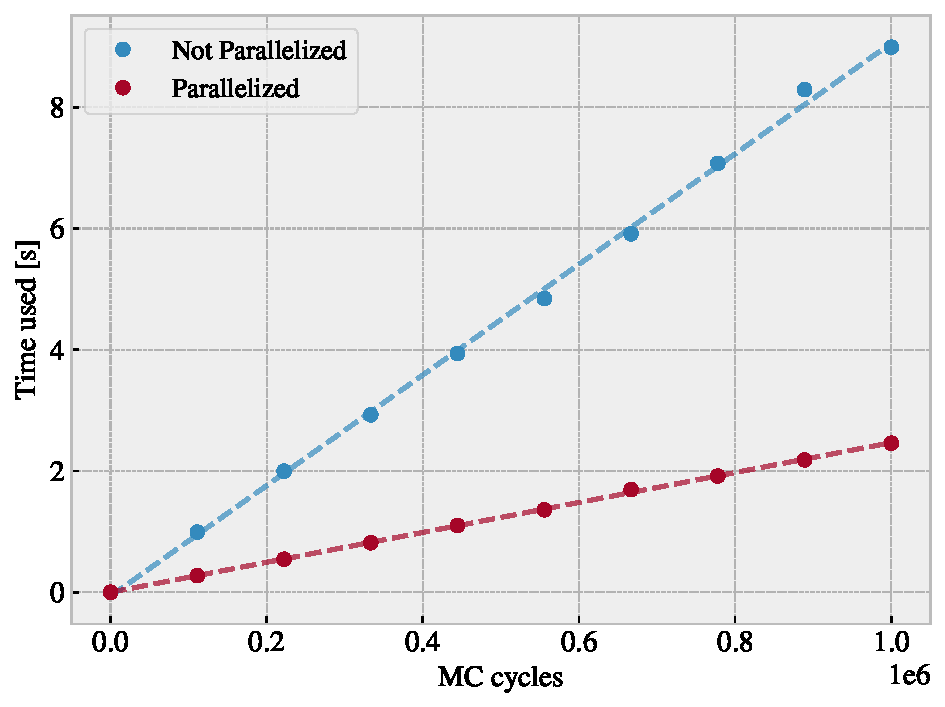
\includegraphics[width=0.45\textwidth]{figures/tmMCcycles.pdf}
  \caption{The time used for the parallelized and non-parallelized code at different numbers of MC cycles. The temperature is kept constant at $T = 1.0 \ k_B/J$ and the total number of cycles at 400 ($20\times20$ lattice). The dotted lines are the best linear fit which yielded a slope of $\num{2.4677e-6}$ for the parallelized code and $\num{9.12207e-6}$ for the non-parallelized code, indicating a  speed-up of 3.70.}
  \label{fig:tmMCcycles}
\end{figure}
 \begin{figure}  
  \centering
  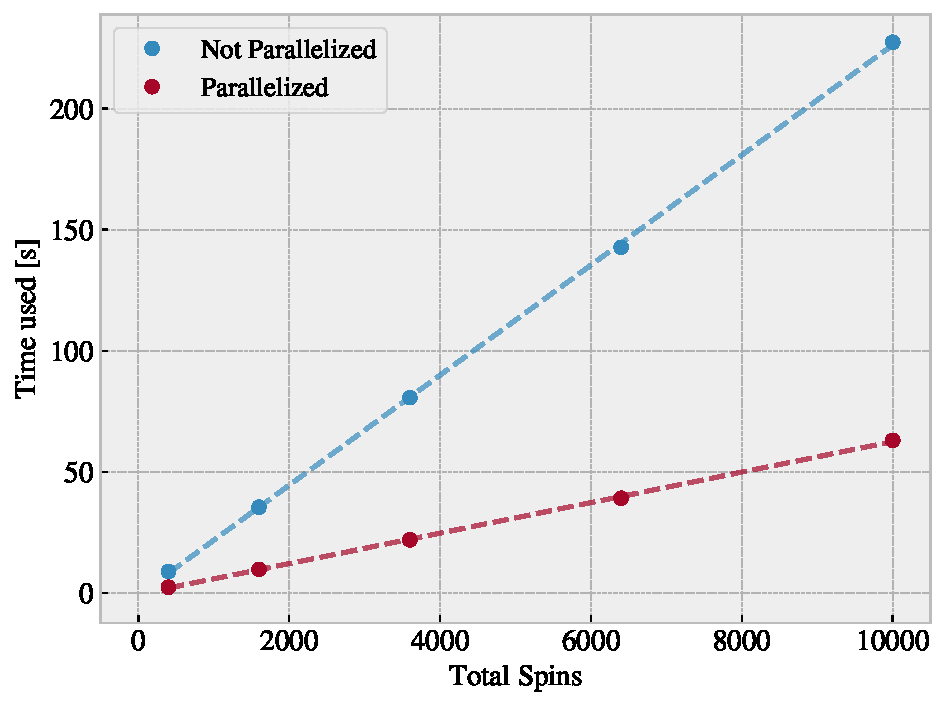
\includegraphics[width=0.45\textwidth]{figures/tmSpins.pdf}
  \caption{The time used for the parallelized and non-parallelized code at different numbers of total spins in the lattice. The system is simulated for $10^6$ MC cycles with a temperature of $T = 1.0 \ k_B/J$. The dotted lines are the best linear fit which yielded a slope of 0.00630 for the parallelized code and 0.02272 non-parallelized code, indicating a  speed-up of 3.61.}
  \label{fig:tmSpins}
 \end{figure}
  \begin{figure}  
  \centering
  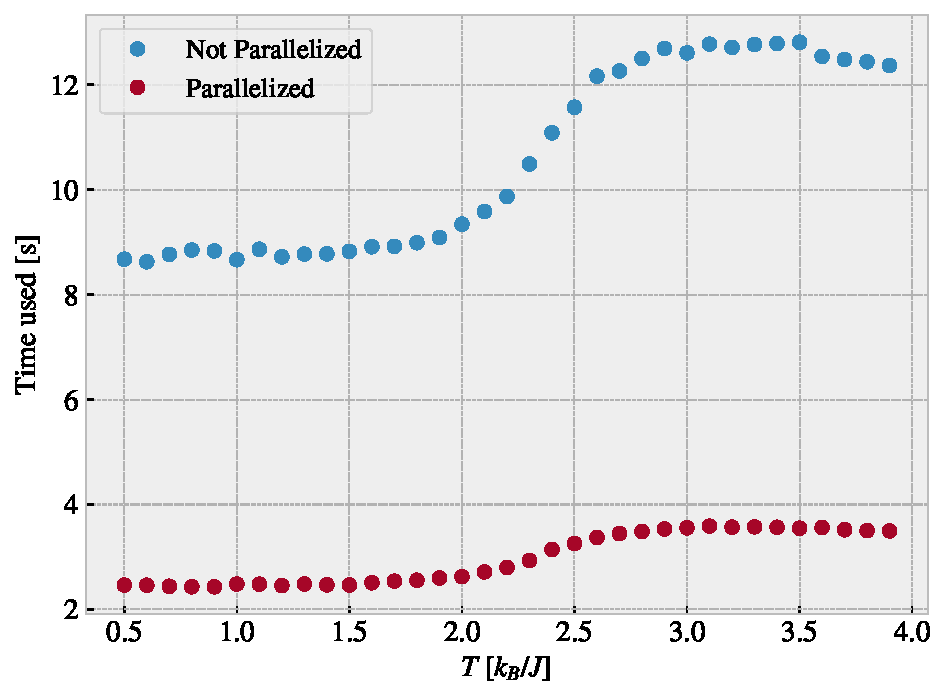
\includegraphics[width=0.40\textwidth]{figures/tmTemp.pdf}
  \caption{The time used for the parallelized and non-parallelized code at different temperatures. We kept the MC cycles at $10^6$ and the total number of cycles at 400 ($20\times20$ lattice). The average factor difference between the two results is 3.56 which indicates the speed-up.} 
  \label{fig:tmTemp}
\end{figure}


\subsection{Phase transitions}
For the purpose of finding the critical temperature we performed a series of simulations in the temperature interval [2.1, 2.4]. We used primarily a temperature step of $dT = 0.01$, but this was decreased to $dT = 0.001$ in the area closer to the critical temperature. We did this for lattice sizes L = 40, 60, 80 and 100. For the initialization of the system we used a configuration with random spin direction. We used $10^5$ cycles to stabilize the lattice before the first time-step and then ran for $10^6$ MC cycles for each time-step. We let the last spin configuration be inherited as the starting point for the simulation on the next temperature step. Again we excluded the data from the first percentage of the MC cycles to make sure that the system had reached its most likely state. We then calculated the expectation values per spin for energy $E$ and absolute magnetization $|M|$ along with the heat capacity $C_V$ and susceptibility $\chi$ which are showed in figure \ref{fig:final_phase}. \\
From the results of the heat capacity and the susceptibility we estimated the temperature corresponding to the maximum value. For this we used a Savitzky–Golay filter (window length = 47, polyorder = 3) to smooth the data points. We then plotted the temperature points against the inverse value of $L$ (see figure \ref{fig:findTc}) in order to estimate the critical temperature for an infinite lattice using equation \ref{eq:findTc}. We achieved the final result showed in table \ref{tab:phase_results}.

\begin{table}[H] 
  \begin{center}
  \caption{Estimated values for the critical temperature $T_C$ for an infinite lattice. This is done by performing linear regression on the data points shown in figure \ref{fig:findTc}, where the estimated value is given as the intercept (see equation \ref{eq:findTc}). By combining the results from the heat capacity and susceptibility we arrive at a mean result where the uncertainty is calculated as $\Delta \overline{T_C} = \sqrt{(\Delta C_V)^2 + (\Delta \chi)^2}$ \\} 
  \begin{tabular}{|c|c|c|} \hline
      & Estimated $T_C$ & \text{Uncertainty} \\ \hline
      Heat capacity & 2.266 & 0.004\\ \hline
      Susceptibility & 2.273 & 0.006\\ \hline
      Mean result & 2.269 & 0.008 \\ \hline
  \end{tabular}
  \label{tab:phase_results}
  \end{center}
\end{table}


\onecolumngrid

 \begin{figure}[H]
  \centering
  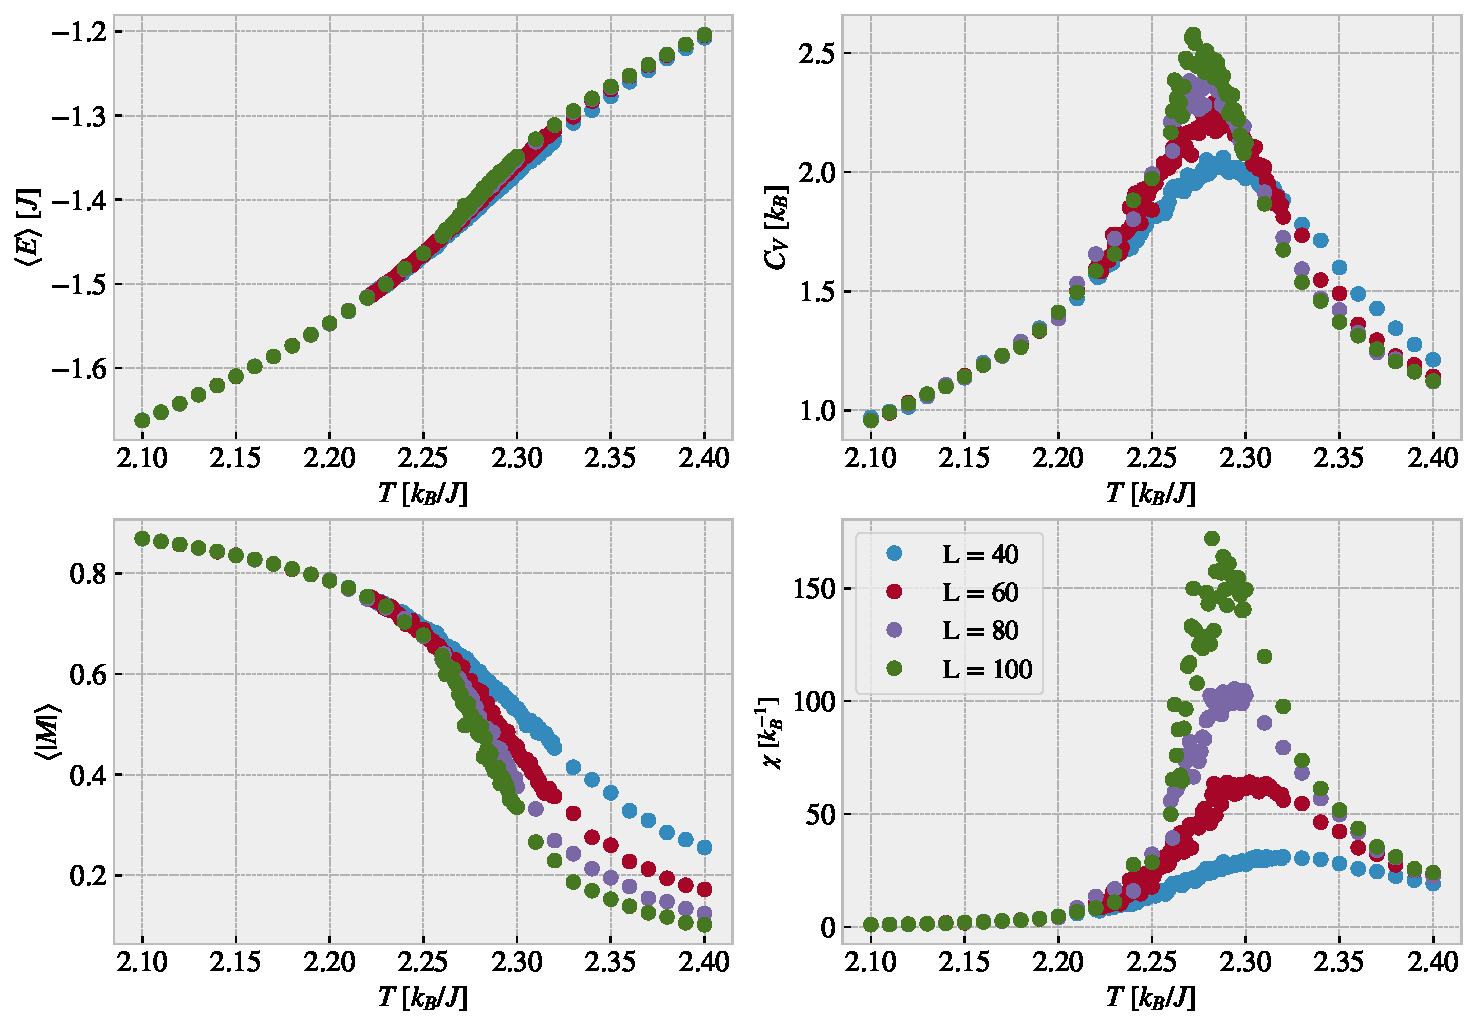
\includegraphics[width=0.9\textwidth]{figures/phase_subplot.pdf}
  \caption{The expectation values per spin for energy $E$, absolute magnetization $|M|$ along with the heat capacity $C_V$ and magnetic susceptibility $\chi$ for different temperatures and with different lattice sizes $L\times L$. We used $10^6$ MC cycles for each temperature step where the first $10^4$ cycles (1\%) of each simulation are excluded from the calculations due to the stabilization time. At the first temperature step the system were initialized with random spin direction, and an additional $10^5$ cycles were used before the first simulation as a safety measure to ensure that the system had reach equilibrium. From there on the last configuration was inherited by the next simulation on the next temperature step. We used primarily a temperature step of $dT = 0.01$, but this was decreased to $dT = 0.001$ in the area around the critical temperature. }
  \label{fig:final_phase}
\end{figure}


\twocolumngrid

 \begin{figure}[H] 
  \centering
  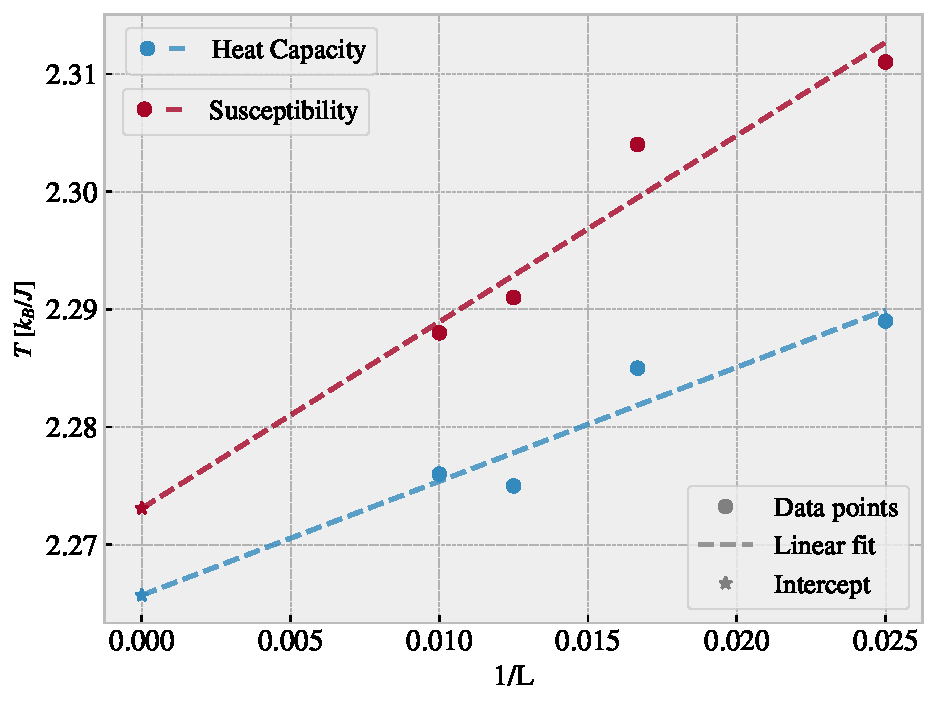
\includegraphics[width=0.45\textwidth]{figures/findTc.pdf}
  \caption{The temperature value corresponding to the maximal value of the heat capacity and the susceptibility as a function of the inverse lattice size $1/L$. By doing linear regression we find an intercept $2.266 \pm 0.004$ for the heat capacity and $2.273 \pm 0.006$ for the susceptibility resulting in an mean value of $2.269 \pm 0.008$.} 
  \label{fig:findTc}
\end{figure}



\section{Discussion}
\subsection{2x2 benchmark}
In figure \ref{fig:equilibrium_benchmark} we can see that the numerical values goes towards the analytical value as the system stabilizes from the chosen initial configuration. It uses approximately $10^4$ MC cycles to reach the most likely state. In figure \ref{fig:phase_benchmark} we also see a very good match between the numerical results and the analytical values as a function of temperature. This is despite the fact that we included the stabilization period where we see that the numerical values deviated from the analytical in figure \ref{fig:equilibrium_benchmark}. Since this deviation is only present for the first $10^4$ cycles (1\%) we understands why it do not effect the overall result noticeable.


\newpage
\subsection{Reaching Equilibrium}\label{sec:reaching_equilibrium}
We see from figure \ref{fig:equilibrium_energy} and \ref{fig:equilibrium_magnetization} that the stabilization of the expectation values of $E$ and $|M|$ for the $20\times 20$ lattice behaves similarly to the case of the $2\times2$ lattice in figure \ref{fig:equilibrium_benchmark}. One main difference is we now see a larger stabilization time of roughly $10^5$ MC cycles. This can mainly be explained by the fact that we have a more complicated system (more possible microstates), but more importantly that we have used different temperatures and initial configurations. If we look at the case of $T = 1.0 \ k_B/J$ we see that the ordered initial configuration is in its most likely state from the beginning, while the initial configuration with random spin directions uses $10^5$ cycles to stabilize. For the latter case we actually see that the expectation values $\langle E \rangle$ and $\langle |M| \rangle$ seemed to stabilize at wrong value (unequal to the final most likely state) for a moment around $\num{1.1e3}$. Then suddenly it drops drastically towards the real most likely value where it becomes consistent with the system that were initialized with an ordered configuration. This shows that certain "bad" starting configurations demand a larger number of cycles in order to stabilize properly. For $T = 2.4 \ k_B/J$ we see that the stabilization time for the ordered and random configuration is almost identical for the $\langle E \rangle$ while the ordered configuration stabilizes a bit faster regarding $\langle M \rangle$. For this observation we must remember that we deal with a random initial configuration and this might not be the case every time.\\
On figure \ref{fig:accepted_spins} we see that the percentage of accepted spins is clearly dependent on the temperature. For a low temperature the acceptance rate is low and for a high temperature the acceptance rate is higher. We know that the Metropolis algorithm uses the criteria $e^{\beta \Delta E} \leq r$, where r is a random number between 0 and 1, to accept the spin. Therefore by raising the temperature we raise the likelihood of the spin acceptance just as the results show.


\subsection{Parallelization / Timing of algorithm}
From figures \ref{fig:tmMCcycles}, \ref{fig:tmSpins} and \ref{fig:tmTemp} we estimated that the parellezation of the code has given a speed-up of $\approx 3.6$. Since we increased the number of cores used from 1 to 4 we expected a speed-up by a factor of 4. The reason why the actual speed-up is a little lower could be due to logistical issues as MPI has to distribute the work to the different cores. In addition we have seen that the time used is linearly dependent of the number of MC cycles and total spins. Since the number of sweeps though the lattice is also linear dependent of those variables this is expected. In the plot of time as a function of temperature (figure \ref{fig:tmTemp}) we see a curve that is similar to the curve in figure \ref{fig:accepted_spins}, where we plotted the accepted spins as a function of temperature. If a spin is accepted we have to update the energy and magnetization as well as updating the boundary conditions. Therefore, the acceptance rate impacts the time used for different temperatures. 

\subsection{Probability distribution}
Figure \ref{fig:energy_distribution} shows two probability distributions, one is narrow with a temperature of $T = 1.0 \ J/k_B$, and the other is broader with a temperature of $T = 2.4 \ J/k_B > T_C$. We see that as the temperature rises, more energy levels become available. From figure \ref{fig:accepted_spins} and the discussion in section \ref{sec:reaching_equilibrium} we know that the acceptance rate increases with temperature. Since the acceptance rate is directly linked with the energy fluctuation, this explains numerically why the model will have a wider energy distribution at a higher temperature level. 


\subsection{The phase transition}
In figure \ref{fig:final_phase} we can see that the heat capacity and susceptibility peak around the expected critical temperature (Onsager: $T_C = 2.269$). As we increase the lattice sizes the peaks get taller and the temperature according to the maximum point goes towards the critical temperature from above. For an infinite lattice, at the thermodynamic limit, we would expect the heat capacity and susceptibility to diverge at the critical temperature. From the observed tendency of the peaks for the heat capacity and susceptibility we get an agreement with this concept. For the expectation value of the absolute magnetization we see that it goes towards zero around the critical temperature. As the lattice size increases this goes faster and faster towards zero. In the thermodynamic limit we expect the magnetization to be zero at the critical point, which then again agrees with the tendency observed. For the expectation value of the energy we see that it is roughly proportional to the temperature. We do not see much change as the lattice sizes increase, but we see some splitting in the curve for different lattice sizes for temperatures just above the expected critical temperature. For higher temperatures the curve meet again making the difference in lattice size irrelevant. This might be explained by looking at the behaviour from the heat capacity. We see that the biggest difference in heat capacity due to different lattice sizes occurs in the temperature interval just after the critical temperature. Since the biggest lattice size has the biggest peak we know that the energy change due to temperature must be biggest for that lattice also. On the other hand the heat capacity for the biggest lattice size seems to drop faster after peaking which result in a lower energy increase per temperature increment in the following intervals compared to the smaller lattices. By combining these observations we can justify that the energy curves meet again after the split.\\
The maximal values of the heat capacity and the susceptibility were used in an approximation of the critical temperature, shown in figure \ref{fig:findTc}. The approximated mean value $\overline{T_C} = 2.269 \pm 0.008$ is consistent with the analytical value by Onsager ($T_C = 2.2692$) within the uncertainties. In the calculation of the uncertainties we only used data from the linear fit. If we included the uncertainty in the determination of the maximum points for the heat capacity and susceptibility we might have gotten a bigger margin of error. We should be skeptical about the use of a Savitzky–Golay filter to smooth the data points. Ideally we would have used more data points to avoid such needs. In addition we believe that the number of MC cycles used were generally on the low side. If granted more computer power one should try this with up to $10^7$ MC cycles and also bigger lattice sizes if possible to support our results even more. None the less we have successfully showcased that our numerical result goes towards the analytical values as the lattice size is increased. This support the fact that the numerical values are true at the thermodynamic limit and of course that the analytical expression from Onsager is correct. 

\newpage
\section{Conclusion}
In this project we have studied the Ising model with the use of the Metropolis algorithm, a Markov chain Monte Carlo method. We started by successfully verifying that our implementation of the model of a $2 \times 2$ lattice were in agreement with the analytical expressions.\\
Then we ran a series of investigations on a $20\times20$ lattice for the stabilization time, accepted spin in the metropolis algorithm as a function of temperature and the energy probability distribution for two different temperatures. We found the general stabilization time to be roughly $10^5$ MC cycles but this differed with the choice of initial configuration and temperature. In general an ordered configuration with all spins aligned proved to be a great choice for $T =1.0 \ k_B/J$, while the configuration for $T = 2.4 \ k_B/J$ did not make a big difference in stabilization time. We saw that the ratio of accepted spins increased with temperature. We also saw that the energy probability distribution widens for higher temperatures which match the observations of the spin acceptance rate.\\ 
In order to get the most efficient code for the simulation of the phase transitions we used MPI to parallelize the program. We saw a $\approx 3.6$ speed-up after paralellizing our algorithm. We verified that the time used is proportional to the number of spins in the lattice times the number of MC cycles. Regarding temperature change we saw that the time used increased for a higher temperature according to the increase in the acceptance rate for spin-flips.\\
For the final part we simulated the phase transition in the temperature interval $T = [2.1, 2.4]$ for lattice sizes $L = 40, 60, 80, 100$. As we increased the lattice size the results changed in direction of the analytical expressions at the thermodynamic limit. By scaling our result we found a mean value for the estimated critical temperature for an infinite 2D lattice to be $T_C = 2.269 \pm 0.008 \ k_B/J$. This is consistent with the analytical value by Onsager ($T_C = 2.2692$) within the uncertainties. With this study we have supported the idea that the numerical values are true in the thermodynamic limit.




\begin{thebibliography}{}
\bibitem{project4} Hoftun F. and Metzsch-Jensen M. (2020), \textit{Project 4 - GitHub repository}, Available at: \url{https://github.com/mikkelme/project4_FYS3150}
\bibitem{project_description} Univeristy of Oslo, Department of Physics (2020) \textit{Project 4 description}, Available at: \url{http://compphysics.github.io/ComputationalPhysics/doc/Projects/2020/Project4/pdf/Project4.pdf}
\bibitem{wiki:Ising} Wikipedia (2020) \textit{Ising model}, Available at: \url{https://en.wikipedia.org/wiki/Ising_model} (Read: November 20th 2020)
\bibitem{Onsager} Onsager L. (1944) \textit{Crystal statistics. I. A two-dimensional model with an order-disorder transition}.  Physical Review, Series II, 65: page 117–149.
\bibitem{wiki:Canonical_ensemble} Wikipedia (2020) \textit{Canonical ensemble}, Available at: \url{https://en.wikipedia.org/wiki/Canonical_ensemble} (Read: November 22th 2020)
\bibitem{fig:style} Haugen I. (2018) \textit{Project 4 - GitHub repository}, Available at: \url{https://github.com/ivarhaugerud/FYS3150/tree/master/project4}
\bibitem{book:fys2160} Schroeder D. V. (2000) \textit{An Introduction to Thermal Physics: Chapter 6}
\end{thebibliography}




%\bibliographystyle{plain}

\clearpage
\section*{Appendix}
GitHub repository: \url{https://github.com/mikkelme/project3_FYS3150}





\subsection{Derivation of the Boltzmann factor\\ and the partition function}
In an isolated system with constant temperature, all the available microstates are equally probable. We then have the relation:
\begin{align*}
    \frac{P(s_2)}{P(s_1)} &= \frac{\Omega (s_2)}{\Omega (s_1)}\\
    &= \frac{e^{S(s_2)/k}}{e^{S(s_1)/k}} = e^{(S(s_2) - S(s_1))/k}
\end{align*}
Where $P(s)$ is the probability of microstate s, $\Omega (s)$ is the multiplicity of microstate s, $S (s)$ is the entropy of microstate s and $k$ is the Boltzmann constant. We used the definition of entropy $S = k \ln \Omega$. We can then utilize the thermodynamic identity
\begin{align*}
    dS &= \frac{1}{T} (dU + PdV - \mu dN)
\end{align*}
Where $T$ is temperature, $U$ is internal energy, $P$ is pressure, $V$ is volume, $\mu$ is the chemical potential and $N$ is the number of particles. In our model the number of particles and volume are constant. This gives us:
\begin{align*}
    S(s_2) - S(s_1) &= \frac{1}{T} (U(s_2) - U(s_1)) = -\frac{1}{T} (E(s_2) - E(s_1)) 
\end{align*}
Where $E(s)$ is the energy of microstate s. We substitute for the entropy:
\begin{align*}
    \frac{P(s_2)}{P(s_1)} &= e^{-(E(s_2) - E(s_1))/kT}\\
    \frac{P(s_2)}{e^{-E(s_2)/kT}} &= \frac{P(s_1)}{e^{-E(s_1)/kT}}\\
    P(s) &= \frac{1}{Z} e^{E(s)/kT}
\end{align*}
Where $e^{E(s)/kT}$ is the Boltzmann factor, $1/Z$ is a normalization constant. The sum of all probabilities must be 1:
\begin{align*}
    \sum_s P(s) &= 1\\
    \rightarrow Z &= \sum_s e^{- \beta E(s)}, \quad \beta = 1/kT
\end{align*}
Where $Z$ is the partition function.


\subsection{Alternative calculations of analytical values}

\subsubsection{Some formulas}
\begin{equation}
    \langle E \rangle = kT^2 \left( \frac{\partial \ln Z}{\partial T} \right) _{V,N}
    \label{eq:<E>_def}
\end{equation}


\begin{equation}
    \langle E \rangle = \sum_{i=1}^M E_iP_i(\beta) = \frac{1}{Z}\sum_{i=1}^M E_ie^{-\beta E_i}
    \label{eq:<E>}
\end{equation}
\begin{equation}
    C_V =\frac{1}{kT^2} \frac{\partial^2\ln{z}}{\partial \beta^2}
    \label{eq:C_V1}
\end{equation}

\begin{align*}
    C_V = \frac{1}{kT}(\langle E^2\rangle - \langle E\rangle^2) = \frac{\sigma_E^2}{kT}
\end{align*}
\begin{align*}
    \sigma_E^2 = (\langle E^2\rangle - \langle E\rangle^2) = \frac{1}{Z}\sum_{i=1}^M E^2_ie^{-\beta E_i} - \left(\frac{1}{Z}\sum_{z=1}^M E_i e^{-\beta E_1}\right)^2
\end{align*}
\\
\begin{equation}
    \langle M \rangle = \sum_{j=1}^M M_iP_i(\beta) = \frac{1}{Z} \sum_i^M M_i e^{-\beta E_i}
    \label{eq:<M>}
\end{equation}
\begin{equation}
    \langle|M|\rangle = \frac{1}{Z}\sum_i^M |M_i|e^{-\beta E_i}
    \label{eq:<|M|>}
\end{equation}
\begin{equation}
    \chi = \frac{1}{kT}\left(\langle M^2 \rangle - \langle M \rangle^2\right) = \frac{\sigma_{M}^2}{kT}
    \label{eq:chi}
\end{equation}
\begin{align*}
    \sigma_{M}^2 = (\langle M^2\rangle - \langle M\rangle^2) = \frac{1}{Z}\sum_{i=1}^M M^2_ie^{-\beta E_i} - \left(\frac{1}{Z}\sum_{z=1}^M M_i e^{-\beta E_1}\right)^2
\end{align*}

\subsubsection{Some analytical calculations}
\begin{align*}
    Z &= 2e^{8J\beta} + 2e^{-8J\beta} + 12e^0 \\
    &= 4\cosh{8J\beta} + 12
\end{align*}
We have used $\cosh{x} = (e^x + e^{-x})/2$. \\
\begin{align*}
    \langle E \rangle = \frac{1}{Z}\sum_i^m E_ie^{-E_i\beta} = \frac{16Je^{-8J\beta} - 16Je^{8J\beta}}{Z} = -32J\frac{\sinh{8J\beta}}{Z}
\end{align*}
We have used $\sinh{x} = (e^x - e^{-x})/2$. \\
\begin{align*}
    C_V =& \frac{1}{kT^2}\frac{\partial^2\ln{z}}{\partial \beta^2} \\
     =& \frac{1}{kT^2}\frac{\partial}{\partial \beta}\frac{-\langle E \rangle}{Z} \\
    =& \frac{1}{kT^2}\frac{\partial}{\partial \beta}(32J\frac{\sinh{8J\beta}}{Z}) \\
    =&  \frac{32}{kT^2}\frac{8J^2\cosh{(8J\beta)}Z - \frac{\partial Z}{\partial \beta}\sinh{(8J\beta)}}{Z^2} \\
    =&  \frac{32J^2}{kT^2}\frac{8\cosh{(8J\beta)}Z -32\sinh^2{(8J\beta)}}{Z^2}
\end{align*}
\begin{align*}
    \langle|M|\rangle &= \frac{1}{Z}\sum_i^m |M_i|e^{-\beta E_i} = \frac{4e^{8J\beta} + 4\cdot2 + 4\cdot2 + 4e^{8J\beta}}{Z} = \frac{8e^{8J\beta} + 16}{Z} \\
 \langle M^2 \rangle &= \frac{16e^{8J\beta} + 4\cdot4 + 4\cdot4 + 16e^{8J\beta}}{Z} = 32\frac{e^{8J\beta} + 1}{Z}
\end{align*}
\begin{align*}
    \chi &= \beta\left(\langle M^2 \rangle - \langle |M| \rangle^2\right) \\
    &= \beta\left(32\frac{e^{8J\beta} + 1}{Z} - (\frac{8e^{8J\beta} + 16}{Z})^2\right) 
\end{align*}



\end{document}

